\providecommand{\atd}{..}
\documentclass[../main.tex]{subfiles}

\begin{document}
    \chapter{BPMN 1}\label{ch:bpmn-1}
    \section{Description}\label{sec:description2}
    In the first process we described the flow of a general report, coming from an hospital. At the very beginning, the facility sends a notification to the civil protection, that evaluates the report received, sending all the needed information to the system. The system computes the data using the right filters and once it is done it sends the raw results back to the user, which will display them in a user-friendly window. The system will then receive feedback based on the results it previously computed: it could be positive (if the information provided were useful and then the user proceeds with the view of the reports) or negative. In the former case, the filters are saved as default one. In the latter case the user will ask again for computation based on other filters that the he must provide.
    Either way, as an advanced feature, the system will launch an instance of training using machine learning techniques in order to improve its predictions in the future.

    \section{BPMN 1 Diagram}\label{sec:bpmn-1-diagram}
    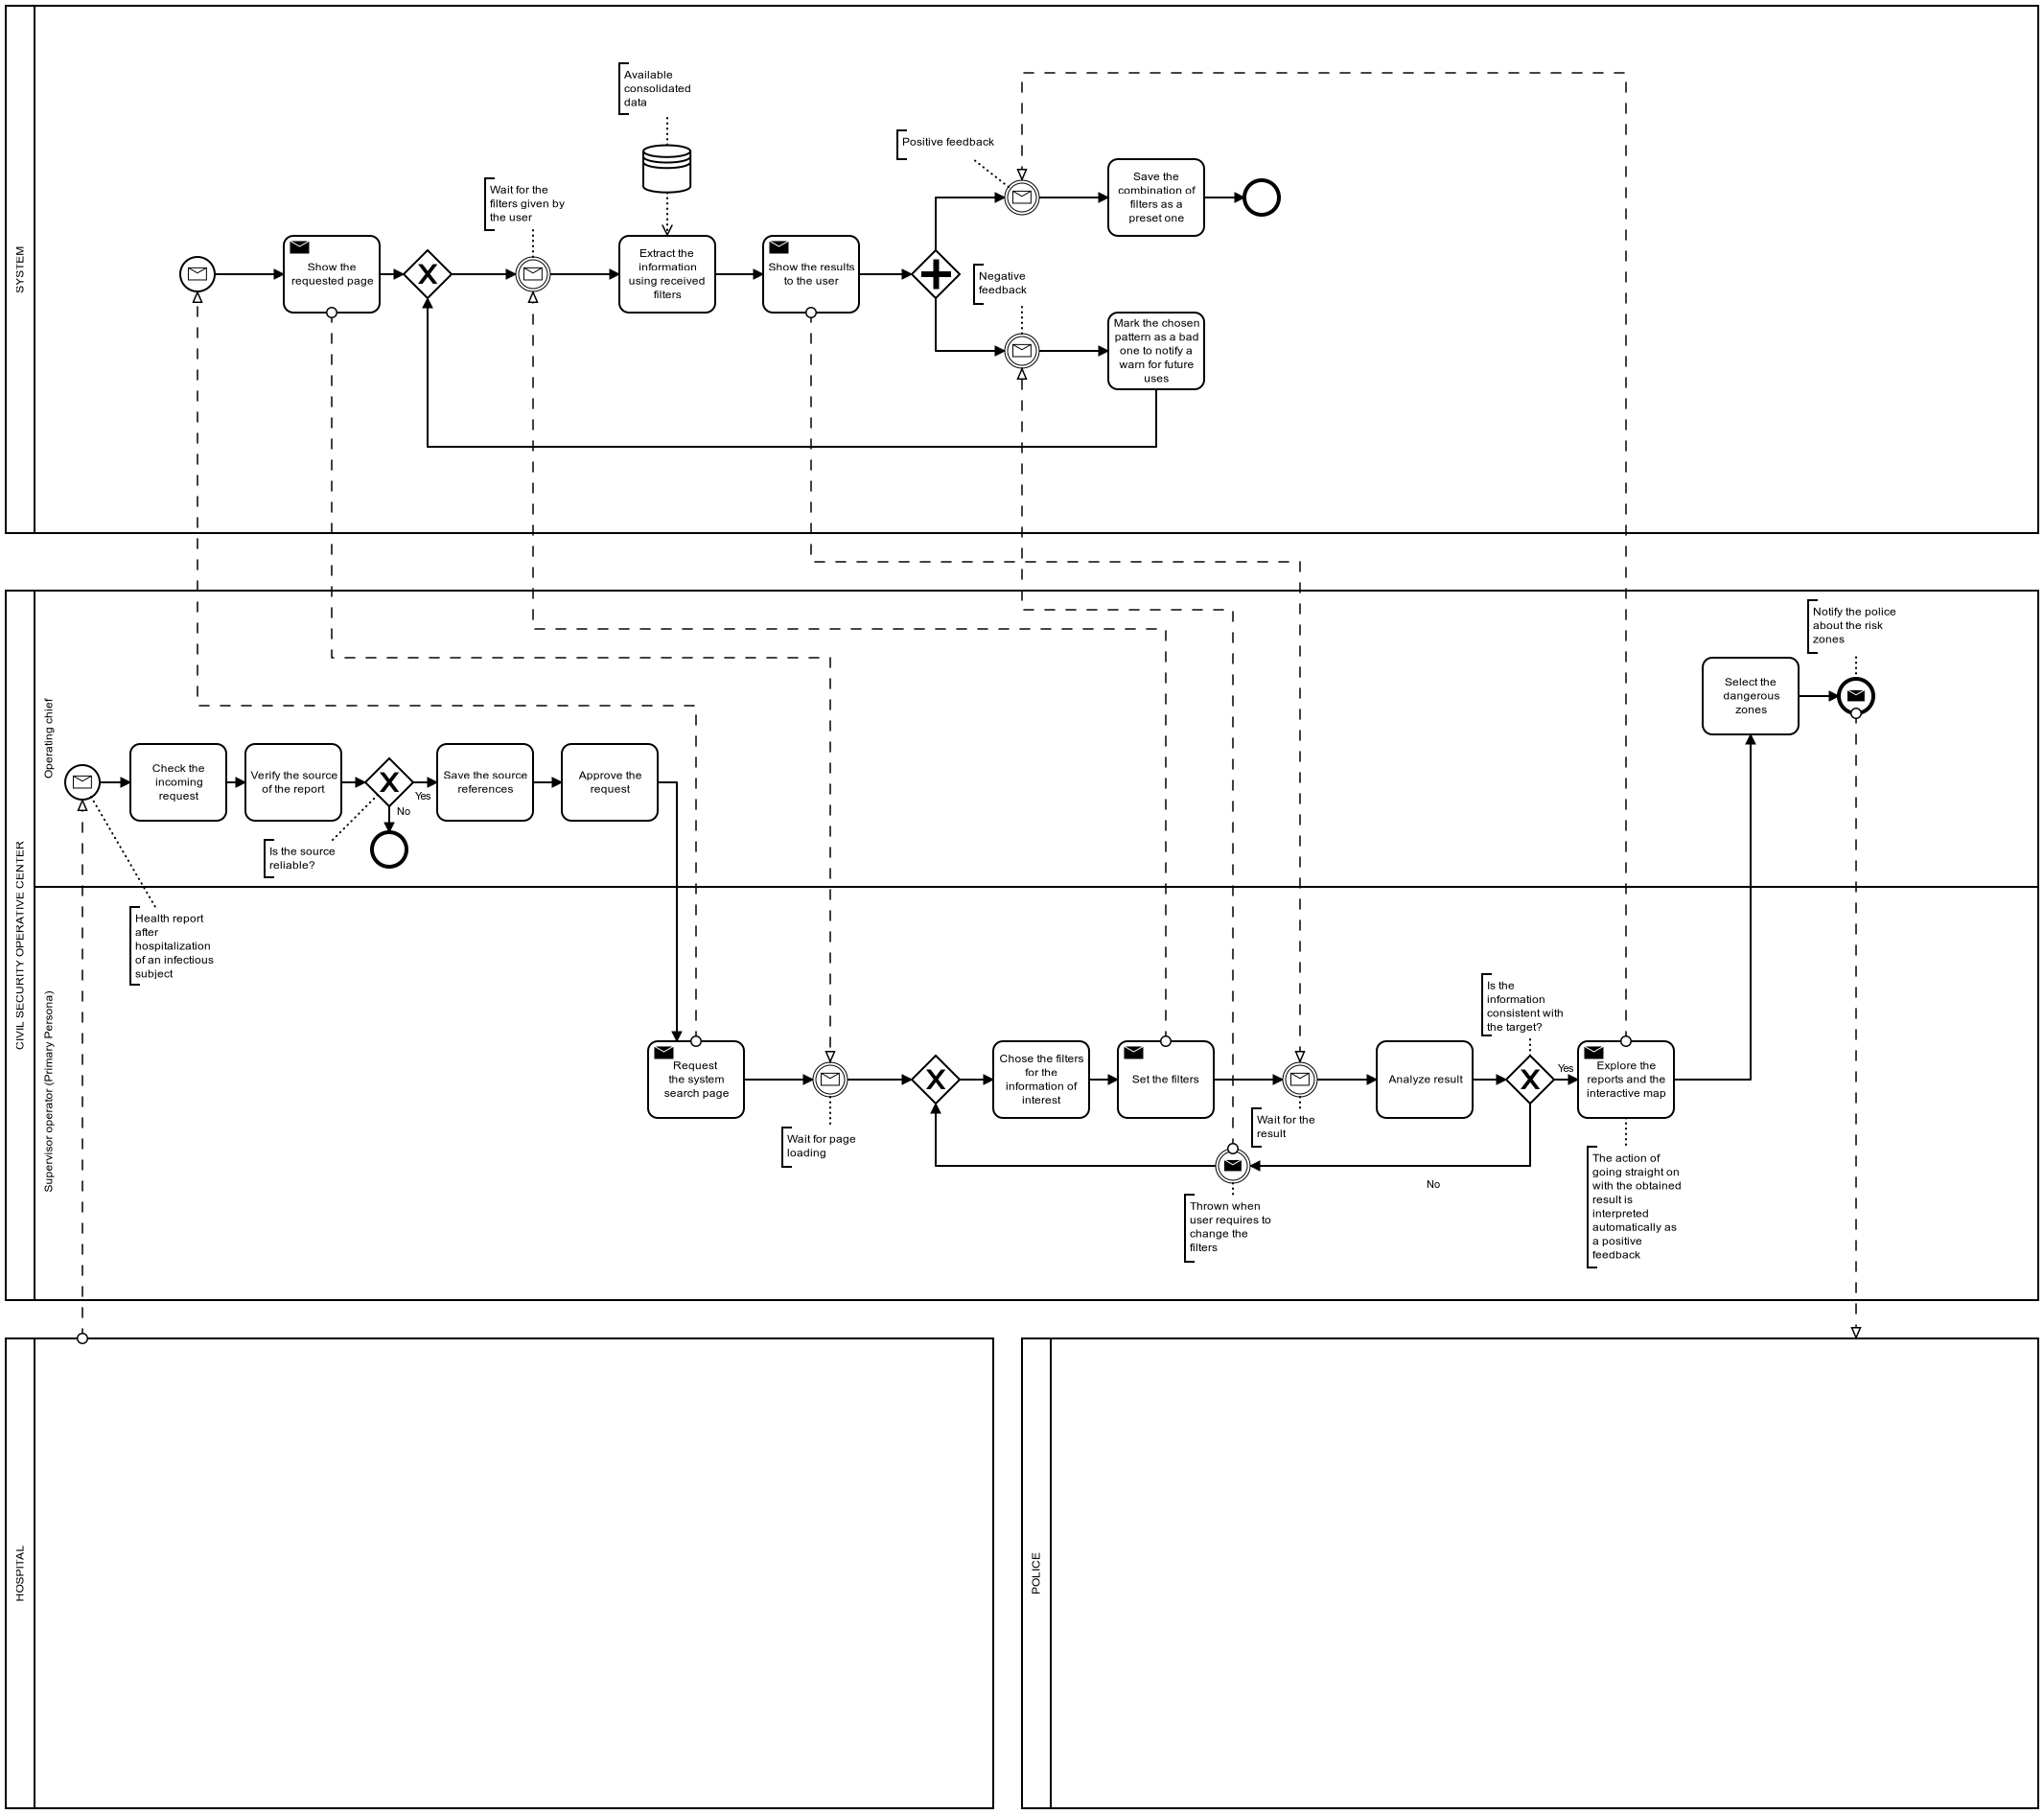
\includegraphics[scale = 0.40]{assets/bpmn1.png}
    \chapter{BPMN 2}\label{ch:bpmn-2}
    \section{Description}\label{sec:description}
    In the second process, we wanted to specify the flow of another important feature of our system: the automated analysis. An analysis can be view as a sort of search that is scheduled to run periodically and aims to check if some constraints are violated.
    An example can be an analysis that checks the crowding level of a station of the public metro transport service of Milan (where data can be acquired from security cameras and turnstiles).
    The analysis is triggered by a specific time event (e.g. every day). The first operation is to fetch the data and then analyze them in order to check whether the given constraints are violated. In this case, it notifies the user through the system. Notice that the “user” is who we have identified as the primary persona. He can decide to ignore the notification and discard it or he can warn his manager (the secondary persona) which can decide the next steps by analyzing the situation: if he decides that the reported situation is not relevant, the process ends.
    Otherwise he proceeds to identify the contact person that has to be informed and then warns him accordingly. In the example, the entity that has to be contacted is the ATM service of Milan, which is represented as a black box from the process point of view: the objective is to be able to identify these situations and warn who is in charge to handle them.
    Another aspect that is highlighted by the process, and which is a key feature of our system, is that these kind of analysis are done, once they are properly configured, in a complete automatic way. The process in fact starts right from the system with a time trigger, and if no particular situations are identified, it ends without involving the user participation.

    \section{BPMN 2 Diagram}\label{sec:bpmn-2-diagram}
    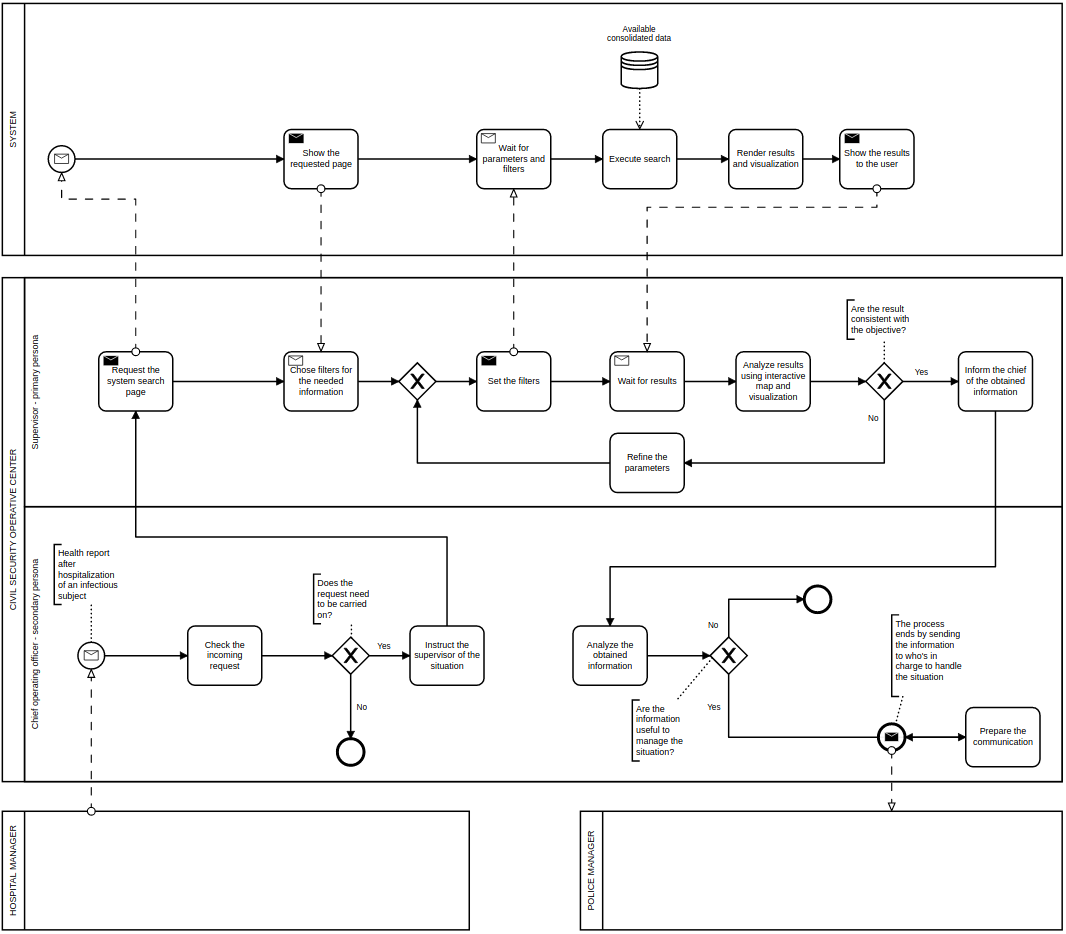
\includegraphics[scale = 0.45]{assets/bpmn2.png}

\end{document}